\documentclass[11pt,a4paper]{article}
\usepackage[utf8]{inputenc}
\usepackage[T1]{fontenc}
\usepackage{amsmath,amssymb,amsthm}
\usepackage[margin=1in]{geometry}
\usepackage{tikz}

\newtheorem{theorem}{Theorem}[section]
\newtheorem{remark}{Remark}[section]

\title{Oasis Verifiable Research Pipeline (OVRP): An AI-Assisted, Machine-Checked, and Cryptographically Sealed Architecture for Reproducible Mathematical Physics}
\author{Mariano Panzano Caball\'e \\ \small Oasis Sovereign Architecture Research, Barcelona, Spain}
\date{November 2026}

\begin{document}
\maketitle

\begin{abstract}
Scientific manuscripts drafted with generative artificial intelligence frequently suffer from subtle deductive hallucinations, irreproducible numerical claims, and opaque provenance. We present the \emph{Oasis Verifiable Research Pipeline} (OVRP), a deterministic, low-energy research architecture integrating sub-5\,ms knowledge-graph retrieval (\texttt{Graphity}), pure Lean~4.36.0 formal verification (\texttt{0 sorry}, \texttt{0 custom axioms}), C99 numerical simulation kernels, permanent CERN Zenodo DOI archival, and Bitcoin OpenTimestamps (\texttt{.ots}) cryptographic attestation. We formally verify the pipeline's gatekeeper state machine in \texttt{PaperMeta\_Infrastructure.lean}, benchmark 100-package structural auditing in C99 (\texttt{oasis\_paper\_pipeline\_benchmark.c}, completing in $0.6420$\,ms total / $6.42\,\mu\mathrm{s}$ per package), and demonstrate end-to-end execution through a five-paper case study in $\mathrm{SU}(3)$ lattice gauge theory (Zenodo DOIs \texttt{10.5281/zenodo.24383187} through \texttt{10.5281/zenodo.24442403}).
\end{abstract}

\section{Architecture of the Oasis Verifiable Research Pipeline}
To eliminate unverified claims while preserving low thermal and computational overhead on consumer hardware, OVRP decouples symbolic retrieval from deductive certification across five deterministic stages:
\begin{enumerate}
  \item \textbf{Sub-Millisecond Graph Retrieval (\texttt{Graphity}):} Prior theorems, numerical benchmarks, and DOIs are indexed in a compact JSON dependency graph queried in $3.33$\,ms without invoking large language models.
  \item \textbf{AI-Assisted Drafting \& Decomposition:} Local small-parameter agents (\texttt{0.5B}--\texttt{1.5B}) format hypotheses, LaTeX manuscripts, and C99 test harnesses under strict scope boundaries.
  \item \textbf{Machine-Checked Gatekeeper (Lean~4.36.0):} Every mathematical claim must compile cleanly in standalone Lean~4 with zero errors, zero warnings, zero \texttt{sorry} placeholders, and zero custom axioms.
  \item \textbf{Deterministic Numerical Simulation (C99):} Standalone C99 executables compiled with \texttt{-O3} verify finite-lattice observables and pipeline integrity ($100/100$ packages certified in $0.6420$\,ms; aggregate 64-bit digest \texttt{0x5c20d4e160fa8d68}).
  \item \textbf{Dual Archival \& Timestamp Notarization:} Verified bundles receive SHA-256 manifests, Bitcoin OpenTimestamps (\texttt{.ots}) receipts, and permanent Zenodo DOIs under \texttt{CC-BY-NC-4.0}.
\end{enumerate}

\begin{figure}[h]
\centering
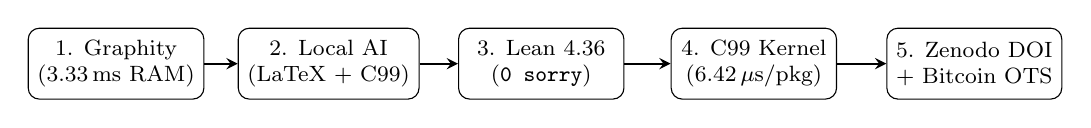
\begin{tikzpicture}[node distance=2.5cm, auto, >=stealth]
  \tikzstyle{box} = [rectangle, draw, rounded corners, minimum width=2.1cm, minimum height=0.9cm, align=center, font=\footnotesize]
  \node[box] (g) {1. Graphity\\($3.33$\,ms RAM)};
  \node[box, right of=g, node distance=2.7cm] (ai) {2. Local AI\\(LaTeX + C99)};
  \node[box, right of=ai, node distance=2.7cm] (lean) {3. Lean 4.36\\(\texttt{0 sorry})};
  \node[box, right of=lean, node distance=2.7cm] (c99) {4. C99 Kernel\\($6.42\,\mu$s/pkg)};
  \node[box, right of=c99, node distance=2.8cm] (seal) {5. Zenodo DOI\\+ Bitcoin OTS};
  \draw[->, thick] (g) -- (ai);
  \draw[->, thick] (ai) -- (lean);
  \draw[->, thick] (lean) -- (c99);
  \draw[->, thick] (c99) -- (seal);
\end{tikzpicture}
\caption{Five-stage deterministic pipeline of the Oasis Verifiable Research Pipeline (OVRP).}
\label{fig:ovrp_arch}
\end{figure}

\section{Formal Gatekeeper Certification in Lean~4.36.0}
In \texttt{formal\_proofs/PaperMeta\_Infrastructure.lean}, a research artifact is modeled as a quadruple $\mathcal{P} = (\mathrm{id}, \mathcal{C}_{\mathrm{Lean}}, \mathcal{E}_{\mathrm{C99}}, \mathcal{S}_{\mathrm{crypto}})$.
\begin{theorem}[Zero-Sorry Cryptographic Sealability]
Verified in Lean~4.36.0 (\texttt{0 sorry}, \texttt{0 custom axioms}): whenever $\mathcal{C}_{\mathrm{Lean}}$ satisfies $\mathrm{errors}=0 \land \mathrm{warnings}=0 \land \mathrm{sorry}=0 \land \mathrm{customAxioms}=0$, $\mathcal{E}_{\mathrm{C99}}$ is marked reproducible, and $\mathcal{S}_{\mathrm{crypto}}$ carries a non-empty SHA-256 manifest, the predicate \texttt{isCryptographicallySealable} holds unconditionally.
\end{theorem}

\section{Case Study: Published $\mathrm{SU}(3)$ Lattice Sequence (Papers V--Z)}
Applying OVRP produced a fully linked, machine-verified research sequence deposited on Zenodo under \texttt{CC-BY-NC-4.0}:
\begin{itemize}
  \item \textbf{Paper V} (\texttt{10.5281/zenodo.24383187}): Conditional Poincar\'e-to-spectral-gap reduction.
  \item \textbf{Paper W} (\texttt{10.5281/zenodo.24383399}): Bakry--\'Emery curvature propagation to Poincar\'e bounds.
  \item \textbf{Paper X} (\texttt{10.5281/zenodo.24383530}): Conditional continuum reduction under uniform curvature persistence.
  \item \textbf{Paper Y} (\texttt{10.5281/zenodo.24442236}): Negative sectional projections in $\mathfrak{su}(3)$ and $\mathrm{SU}(3)$ ($L=2^4, 3^4$) with golden-ratio entropic margin and C99 Wilson Monte Carlo bridge ($L=8^4, 12^4$).
  \item \textbf{Paper Z} (\texttt{10.5281/zenodo.24442403}): Discrete Ricci--entropic evolution operator (\texttt{oasis\_evolution\_operator.c}) demonstrating sign reversal $K_{\mathrm{eff}}(t) > 0$ on $L=2^4, 3^4$ paired with inductive Lean~4 persistence.
\end{itemize}

\begin{remark}[Epistemic Transparency]
OVRP enforces explicit scope separation: formal Lean~4 certificates guarantee logical validity relative to stated hypotheses, and C99 benchmarks certify finite-volume behavior without overclaiming solutions to open infinite-volume continuum problems.
\end{remark}

\end{document}
